% W2 / AC-3.* vibrato spectrograms, hear panel, WT diversity gallery
% Included from main.tex (separate file to reduce merge risk with T2/T3 Methods edits).

\FloatBarrier

\subsection{Vibrato spectrograms}
\label{sec:vibrato-eval}

Do wrap-seam differences stay visible under slow vibrato, beyond static tiled periods?
Figure~\ref{fig:vibrato-spectrogram} renders the same holdout cracked period, DualCosine bake, and refit \textbf{Ours (hybrid GA--PPO)} champion under shared sinusoidal vibrato ($\pm 3\%$ depth at $5$\,Hz around $220$\,Hz).
Panels (a--c) show magnitude spectrograms. Panels (d--e) show DualCosine$-$no-bake and Ours$-$no-bake differences. Panel (g) reports cycle-local prolonged $R$ alongside a modulated-playback residual under the same pitch envelope.
On the annotated high-wrap tile, Ours retains high cycle $R$ and high modulated $R$, while DualCosine remains the weakest classical comparator.
This is objective spectrogram / residual evidence only.
It is not a formal listening study.
Protocol:
\href{https://github.com/reeldemo/reelsynth/blob/main/scripts/bench_vibrato_spectrogram.py}{\texttt{bench\_vibrato\_spectrogram.py}}.
Artifacts:
\href{https://github.com/reeldemo/reelsynth/tree/main/brand/artifacts/vibrato_spectrogram}{vibrato folder}.

\begin{figure*}[t]
  \centering
  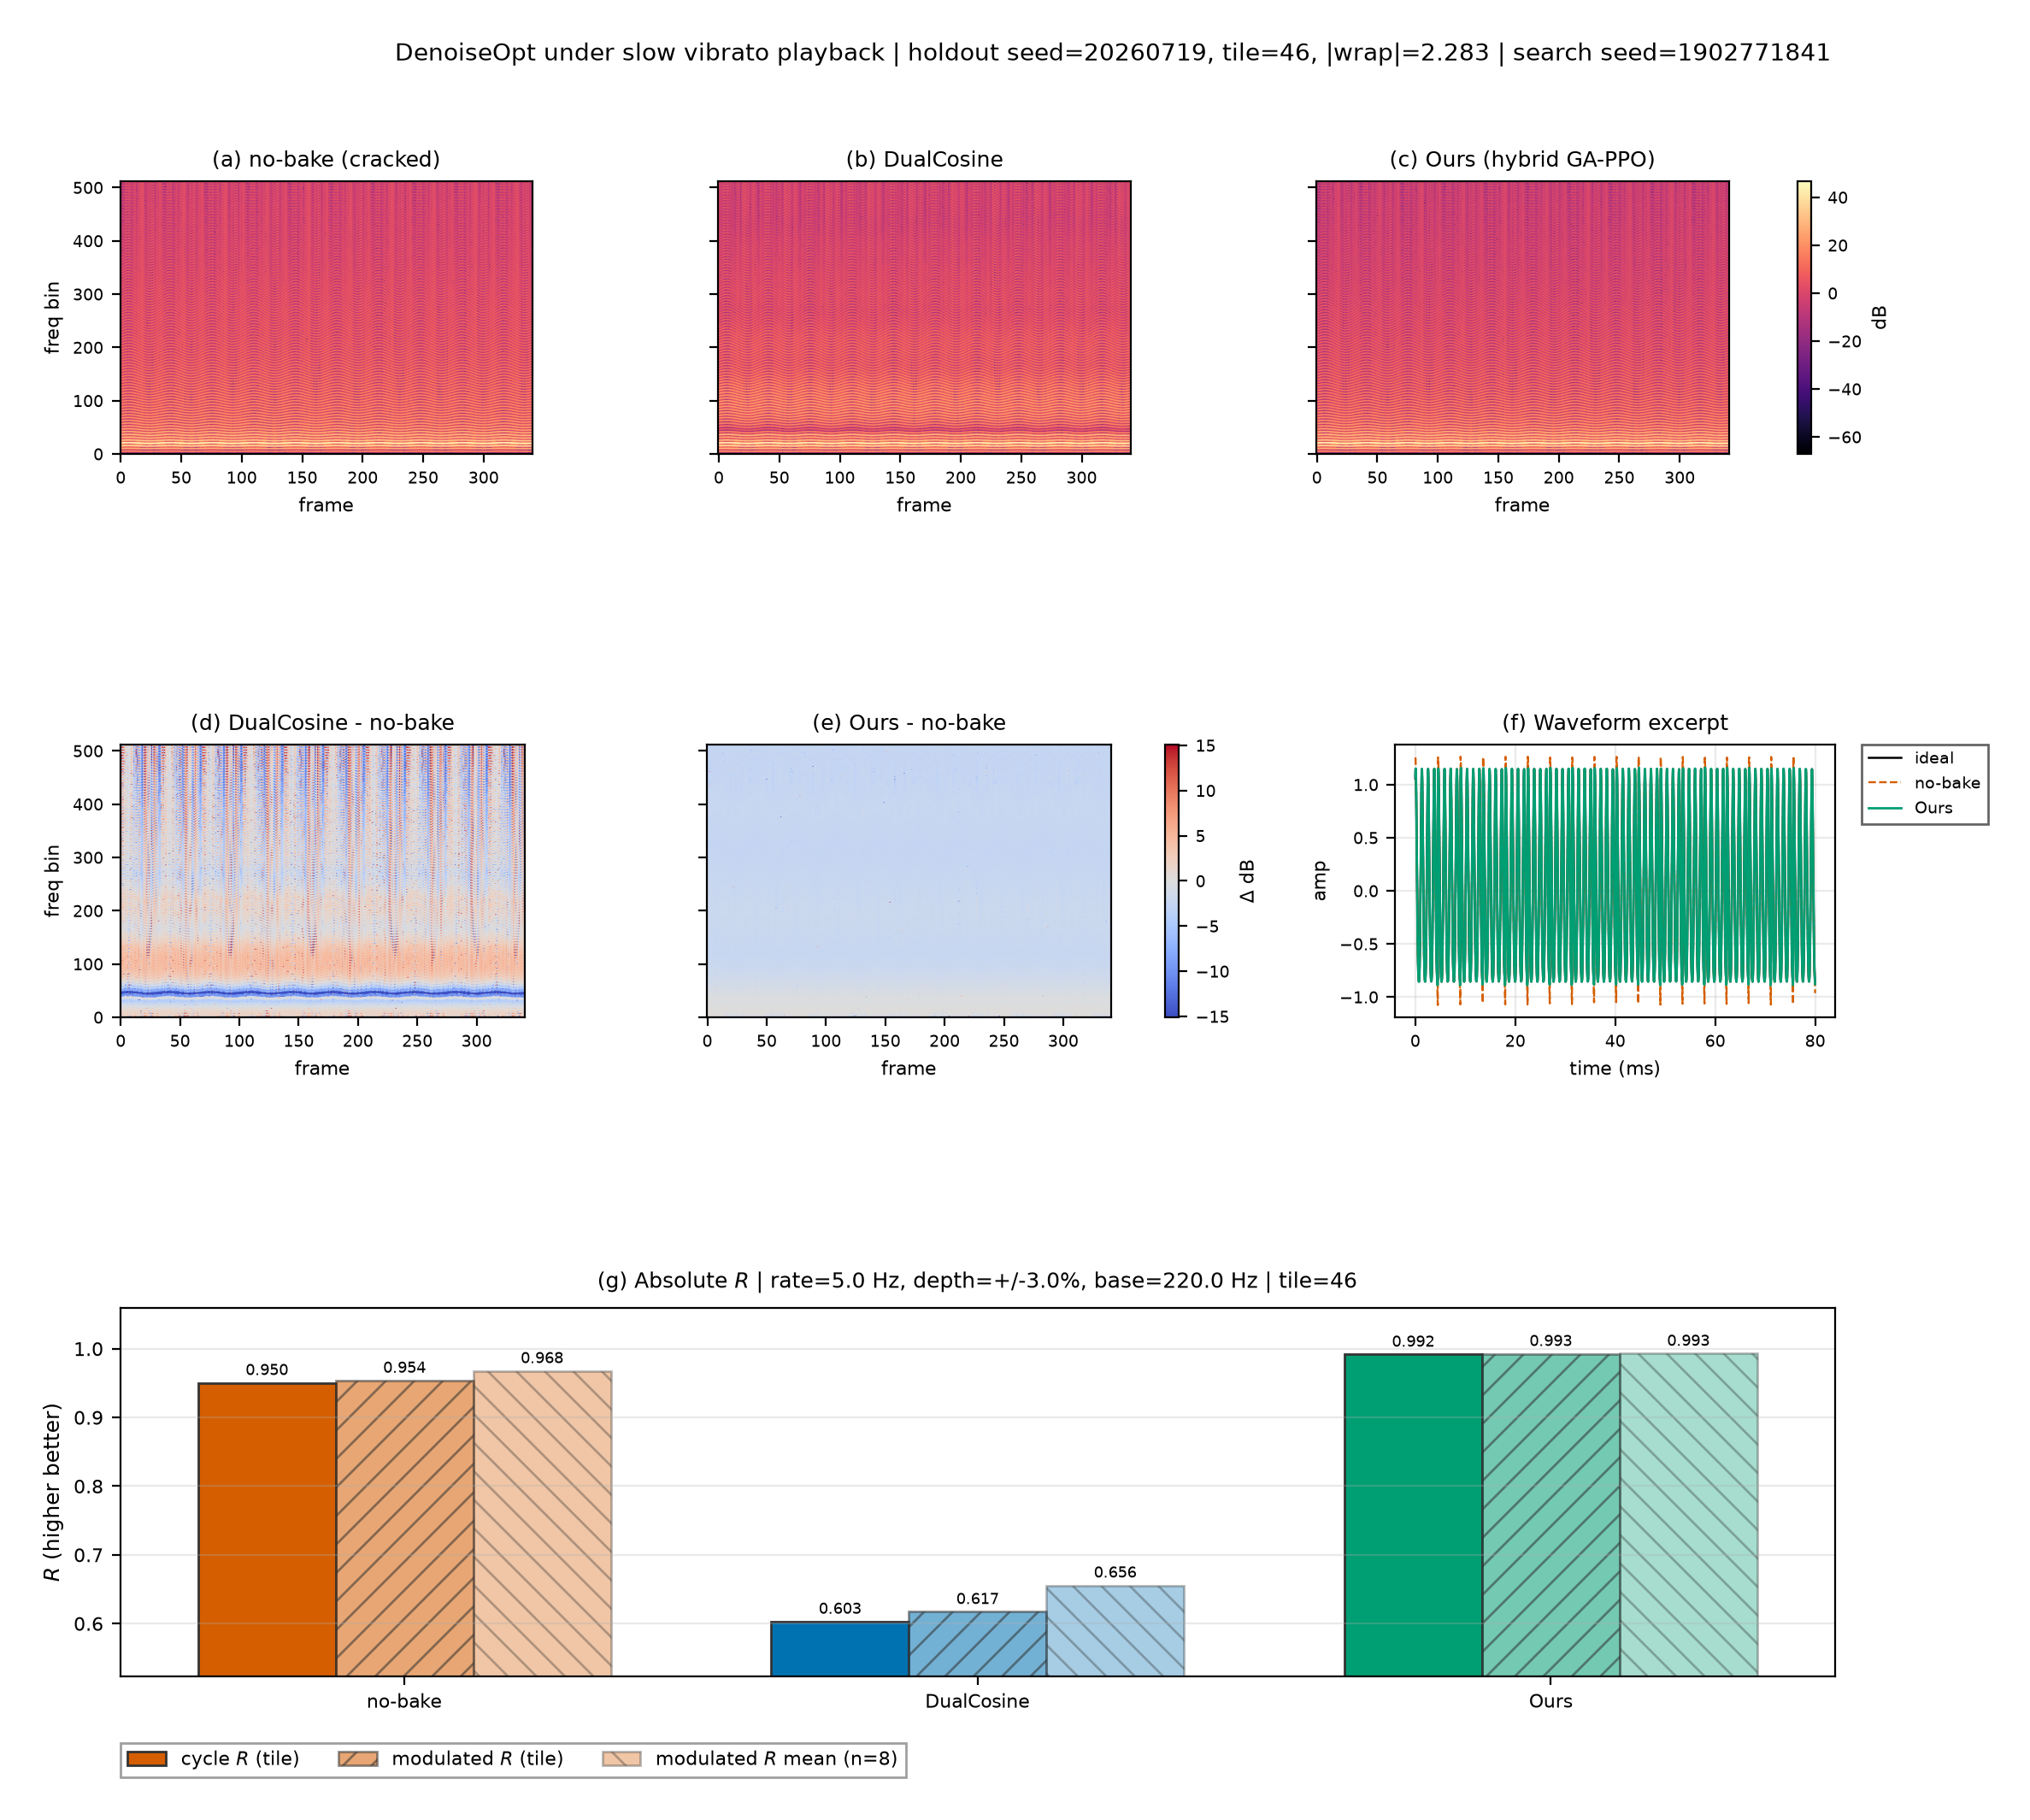
\includegraphics[width=\textwidth]{figures/fig_vibrato_spectrogram.png}
  \caption{Slow-vibrato spectrogram eval on a high-wrap holdout tile (seed~\texttt{20260719}).
    (a--c)~Magnitude spectrograms for no-bake, DualCosine, and Ours.
    (d--e)~Spectrogram differences vs no-bake.
    (f)~Short waveform excerpt.
    (g)~Absolute $R$: cycle-local prolonged residual, modulated-playback residual on the same tile, and mean modulated $R$ over top-wrap tiles.
    Accessibility: Okabe--Ito hues. Difference maps use diverging coolwarm.
    Formal human A/B scores are out of scope.}
  \label{fig:vibrato-spectrogram}
\end{figure*}

\subsection{Downloadable audio samples}
\label{sec:hear-samples}

As an audible companion to Figure~\ref{fig:meta-heal-samples}, we release five fixed-pitch (A4, $3$\,s, $44.1$\,kHz mono) wavetable clips for no-bake, DualCosine, and Ours-healed periods from the matched-suite holdout
(\href{https://github.com/reeldemo/reelsynth/tree/main/brand/artifacts/meta_approach_compare/hear_samples}{hear-sample WAVs},
rebuild:
\href{https://github.com/reeldemo/reelsynth/blob/main/scripts/export_meta_hear_samples.py}{\texttt{export\_meta\_hear\_samples.py}}).
Figure~\ref{fig:hear-samples-panel} shows short waveform excerpts from those WAVs with per-clip absolute $R$.

\paragraph{Listening statistics (null study).}
Table~\ref{tab:listening-stats} is the complete statistical statement for human listening in this paper.
Assumptions: no IRB-recruited listeners; no forced-choice protocol executed; WAV pack is for optional informal inspection of the same tiles already scored by $R_{\mathrm{blend}}$.
Therefore preference mean, std, CI, and $p$-values are undefined (not omitted by accident).
Subjective quality is \emph{out of scope}; objective residual is the claim.

\begin{table}[t]
  \centering
  \caption{Listening / subjective evaluation statistics for this manuscript (honest null study).}
  \label{tab:listening-stats}
  \setlength{\tabcolsep}{6pt}
  \begin{adjustbox}{max width=\columnwidth}
\begin{tabular}{@{}lr@{}}
    \toprule
    Quantity & Value \\
    \midrule
    $N_{\mathrm{listeners}}$ & $0$ \\
    MOS / MUSHRA trials & $0$ \\
    Forced-choice A/B trials & $0$ \\
    Preference mean$\pm$std & n/a (undefined) \\
    Significance tests on preference & none \\
    Released informal WAVs & $15$ ($5$ tiles $\times$ $3$ methods) \\
    Primary quality metric & locked $R_{\mathrm{blend}}$ \\
    \bottomrule
  \end{tabular}
\end{adjustbox}
\end{table}

\FloatBarrier


\begin{figure*}[htbp]
  \centering
  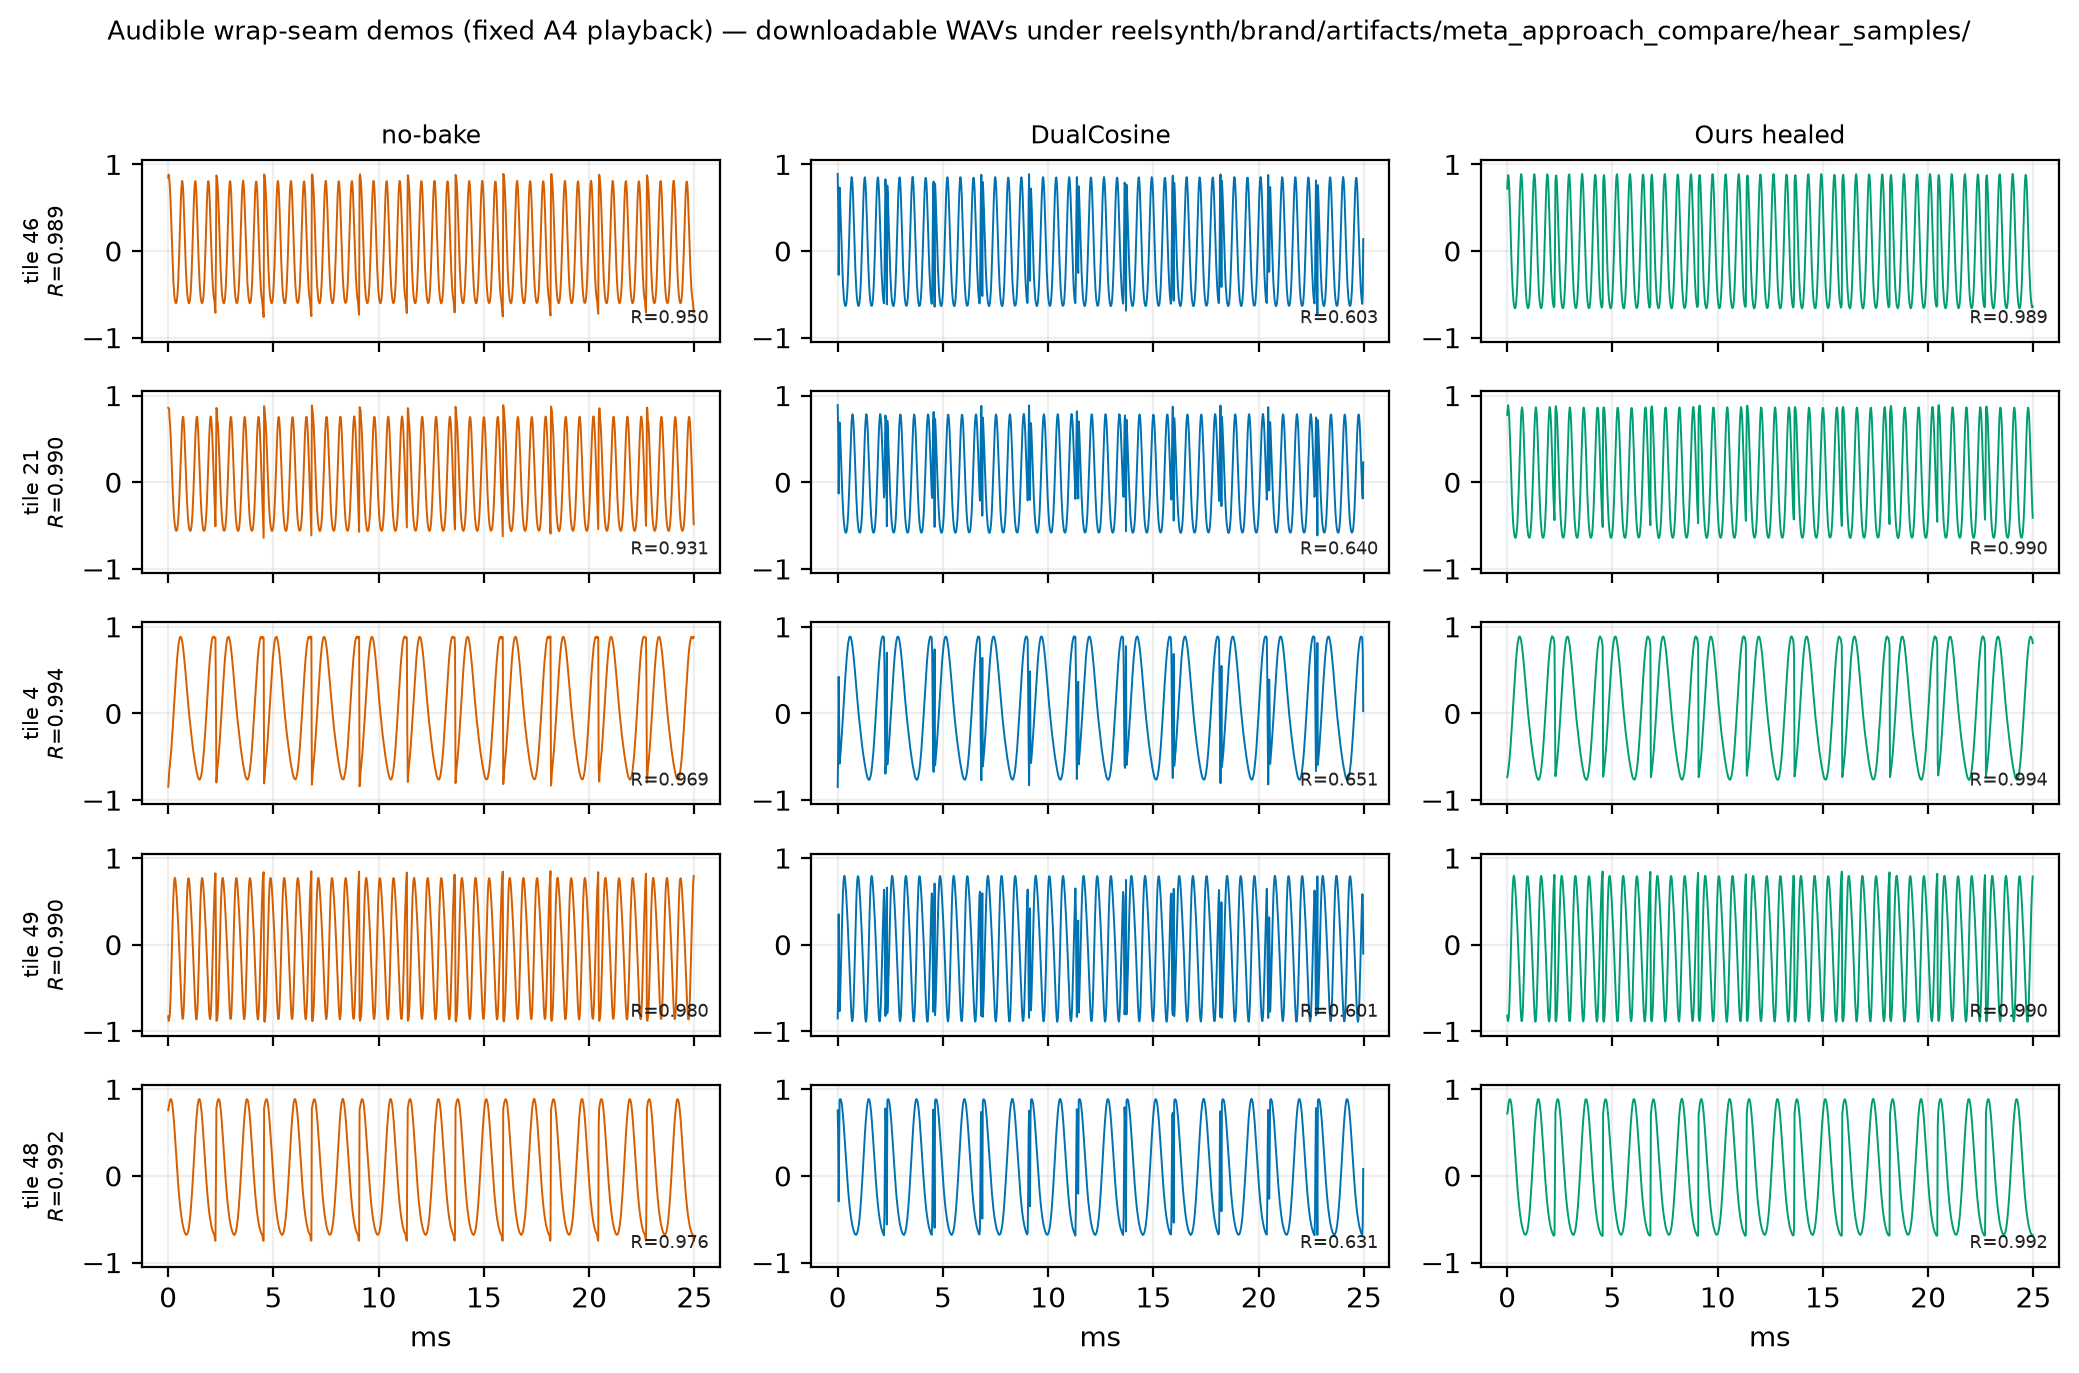
\includegraphics[width=\textwidth]{figures/fig_hear_samples_panel.png}
  \caption{Hear-sample panel from the online WAV pack
    (\href{https://github.com/reeldemo/reelsynth/tree/main/brand/artifacts/meta_approach_compare/hear_samples}{hear-sample WAVs},
    five holdout tiles, no-bake / DualCosine / Ours).
    Waveforms show the first $\approx 25$\,ms of each clip. $R$ annotations are cycle-local prolonged residuals vs the ideal sibling.
    Not a formal listening study.}
  \label{fig:hear-samples-panel}
\end{figure*}

\subsection{Factory and Adventure Kid waveform examples}
\label{sec:wt-gallery}

Beyond the synthetic sine{+}cliff narrative, Figure~\ref{fig:wt-diversity-gallery} shows a compact gallery of true ReelSynth-exported factory periods (one mid-morph frame per bank) and Adventure Kid Waveforms (AKWF) CC0 single-cycle files already used by the wrap protocol.
Scored means remain in Table~\ref{tab:real-wt} and the \href{https://github.com/reeldemo/denoise-opt-meta/blob/master/paper/Unsupervised_Wrap-Discontinuity_Repair_in_Wavetable_Synthesis_via_Hybrid_GA-PPO_Meta-Search_v12/figures/real_wt_matrix.json}{wavetable results}. This panel is diversity evidence only.
No new NAS was run for the gallery.

\begin{figure*}[t]
  \centering
  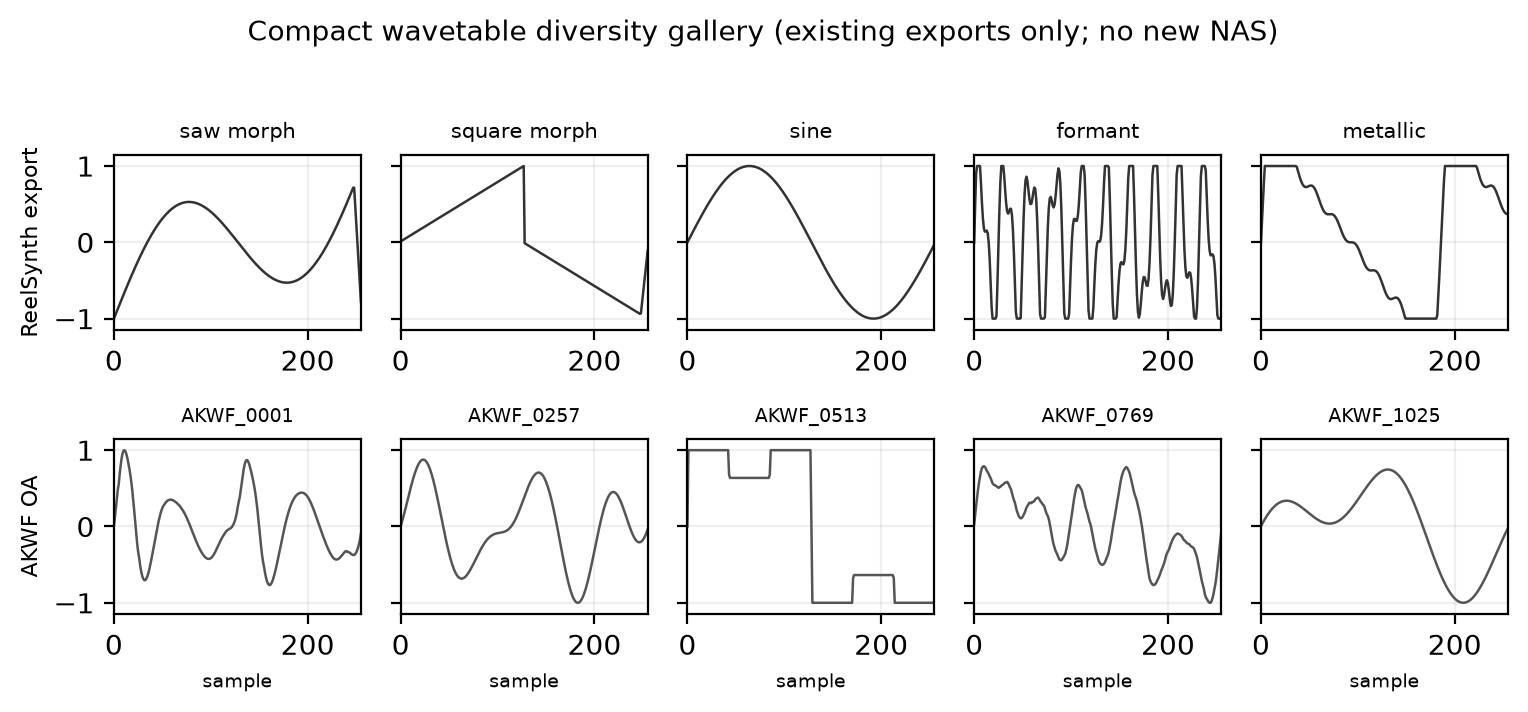
\includegraphics[width=\textwidth]{figures/fig_wt_diversity_gallery.png}
  \caption{Compact wavetable diversity gallery from existing exports
    (one mid-morph dry frame per unique ReelSynth factory bank, top, and matched AKWF CC0 cycles, bottom).
    No new NAS for this panel. Quantitative wrap scores: Table~\ref{tab:real-wt}.}
  \label{fig:wt-diversity-gallery}
\end{figure*}
